\section{Theory}
The theory proposes an IDE-based code completion approach for assisting on writing API sentences. This includes a method to build an API sentence model using an n-gram language model. The main building parts can be seen in (LINK TO IMAGE OVERVIEW). 
To provide a recommendation system for code completion it is needed to mine different source code repositories where the API was used. First the API vocabulary has to be determined in order to extract the corresponding API sentences. With these sentences the API language Model can then be built with the extracted information. The N Gram language model can then recommend proposals taking into account the code that is being edited \cite{Santos2017stepwise}. 

(IMAGE ALL COMPONENTS THAT ARE NEEDED)

There are two core processes to set up the recommendation system for specific API's. First there is the sentence Extractor, as can be seen in (LINK TO IMAGE OVERVIEW). It mines a set of API sentences. Then there is the Model Builder component, which uses these API sentences and builds the API sentence model. Then the model is used by a recommender component in an IDE to assist with the proposals for the user agent. The paper from Santos used the Eclipse code completion system. It uses the context from the user to determine the proposed next Token \cite{Santos2017stepwise}. 
\subsection{Extracting the API sentence}
The sentence extractor is a parser of Java source files and are based on the API of SWT \cite{Santos2017stepwise}. 

In the realm of an API a token is a possible code instruction that includes a public API type and a public operation. Tokens can be seen as abstract representation of code instructions. A set of tokens forms the vocabulary of the API. Three kinds of tokens were considered in the paper: constructor invocation, static operations and instance operations \cite{Santos2017stepwise}. 

A sentence is therefore a sequence of tokens that have a relation to each other. These API sentences are then used to build the language model. The API sentences are mined by parsing every method instruction block \cite{Santos2017stepwise}. 

When mining the API tokens there exist different composite expressions. These expressions were decomposed and treated as having separate instructions. Additionally conditionals and loops are also extracted for each possible branch that they span. The extracted sentence follows the execution order with alternative execution sequences. This includes loops which are treated as if they were conditionals and preserve the execution order \cite{Santos2017stepwise}. 

\subsection{API sentence Model}
The model builder builds the API n-gram language model from the API sentences. The language model is a statistical model that allows to compute probabilities of a sentence depending on the tokens and is able to predict the next word in a sentence for a given language. A language model has a probability distribution over the API sentences. 
\cite{Santos2017stepwise}



\begin{figure}[h]
	\centering
	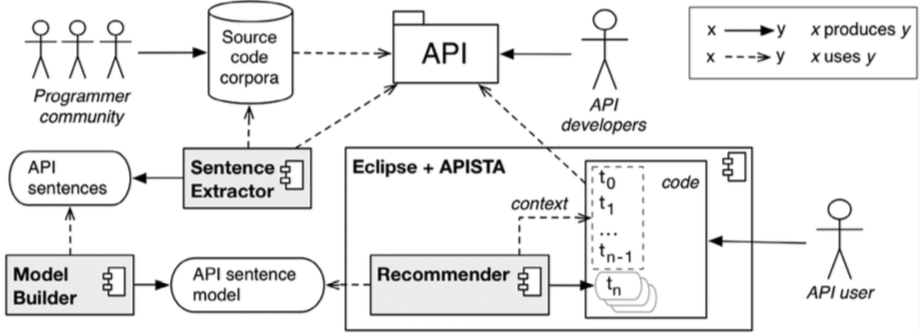
\includegraphics[height=1in]{./section-chapter1/images/overview.png}
	\caption{Overview of model}
	\label{fig:overview}
\end{figure}